% For help on subfiles see https://www.sharelatex.com/learn/Multi-file_LaTeX_projects
\documentclass[../main.tex]{subfile}

\begin{document}
	\section{Introduction}\label{sec::intorduction}
	\paragraph{} Fundamentally, the concept of emulator detection is rooted in the fact that complete system emulation is an arduous task. By discovering or observing differences between virtual and physical execution an attacker can create software virtualization checks that can be used to alter overall program behavior. Such differences may be an artifact of hardware state not correctly implemented in the virtual CPU, hardware or software components that have yet to be virtualized, or observable execution duration \cite{vidas2014evading}
	\paragraph{} Emulator detection and anti-emulator detection is an interesting area of research because its a continuous arms race on both ends. There are some valid reasons for developers to employ emulator detection techniques into their apps and these same techniques can easily be applied by malicious actors to avoid detection or analysis. But on the other hand there are valid reasons for researchers to check for apps that uses emulation detection to hide their true face. Because of the popularity and wide use of Android based smartphones, we felt the urge to study the common tricks and techniques that are used today in this area. Before diving into detailed discussion on these techniques, we will first introduce emulator detection and anti-emulator detection. Then at the end of this chapter we will show some results from our own application that can be used to test emualtor against some detection techniques.

	\subsection{Emulator Detection or Evasion}\label{sec::emu_detection}
	\paragraph{} Its the technique that used by malicious or no malicious applications to detect whether its being executed in emulated environment. The goal of employing this technique is to change the behavior of the application if its being executed inside an emulator. Malicious actors can use this technique to avoid analysis or detection. Non Malicious actors can use it to protect their intellectual property or to stop illegal access to premium features in apps or games.
	
	\section{Anti-Emulator Detection or Cloaking}\label{sec::anti_emu_detection}
	\paragraph{} On the other hand there are people (mostly security researchers) who wants to know what an application is doing and mostly the use emulators to do the analysis of applications. Now an app that uses emulator detection techniques, its not possible to see the actual behavior of this application. In order to solve this problem, anti-emulator detection techniques are used that tries to evade the emulator detection checks and thus the application will be executed as it should on a real device. We would like to note here that due to time constraints we couldn't explore this topic as much as we would have liked to. This topic seems to be not well researched that much and we can recommend a study to come up with solutions on how to cloak against applications that checks for emulator.\todo[inline]{future work} At the end we would like to mention a very interesting approach that is discussed in \cite{rasthofer2016harvesting} which is based on splitting an APK to multiple smaller apks and then dynamically analyzing these smaller apks, furthermore cuckoodroid does have an xposed framework module installed that is called "Android Blue Pill" and during its reversing we found out that it is hooking some of the methods that are commonly used for emulation detection. We tried figuring out the exactly how many techniques it uses to cloak the emulator but there was no information available online and we didn't wanted to spend more time reversing it.
	
	\section{Common emulation Detection or evasion Methods}\label{sec::common_methods_detection}
	\paragraph{} In this section we will describe some of the well known techniques used for emulator detection and will present a list of the emulator detection techniques that was the result of our thorough research on the internet.

	\paragraph{} A general introduction to some of well known techniques can be found in \cite{geist2016jailbreak} and readers are encouraged to have a look at it. There is also another category of detection techniques that can be used in conjunction with emulator detection. These are called root detection and some of these techniques are described in \cite{sun2015android}. These techniques can be easily evaded by using method hooking as demonstarted by \cite{lim2016android}. Figure \ref{fig:root_detection} from \cite{lim2016android} lists the root detection techniques presented in \cite{sun2015android}. There are also several open source packages on github which provides very easy to integrate root checking capibilities to android application, one such example is "root beer" \cite{rootbeer}
	
	\begin{figure}
		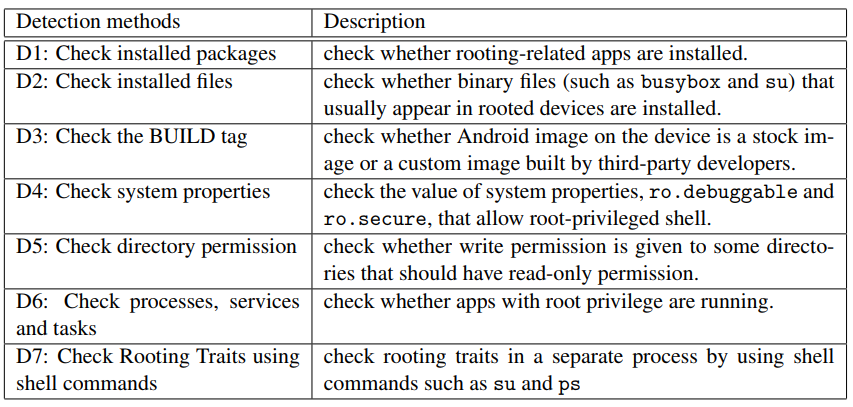
\includegraphics[width=\textwidth]{root_detection.png}
		\caption{Root detection techniques \cite{lim2016android} \cite{sun2015android}}
		\label{fig:root_detection}			
	\end{figure}

	\paragraph{} The paper \cite{lim2016android} also present its own approach to avoid analysis or reverse engineering. They use a stub dex file which contains all of emulation detection code, root detection code. The repackaged the APK so that it loads the stub dex first, which performs emulator checking and if it detects no emulation, then it loads the original dex file otherwise it doesn't load the original dex file.
	\begin{figure}
		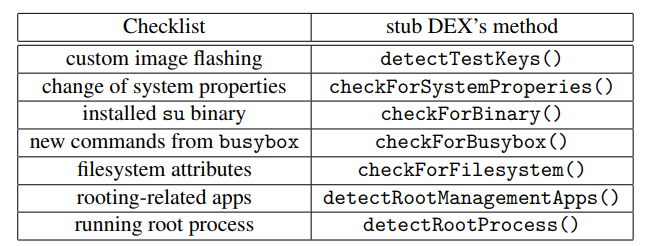
\includegraphics[width=\textwidth]{stub_dex_methods.png}
		\caption{Methods in stub dex \cite{lim2016android}}
		\label{fig:stub_dex_methods}			
	\end{figure}
	They use an effective detection scheme called "call stack analysis" which can be used to detect method hooking and the application is then terminated. For more details on this topic, have a look at section \ref{sec::hooking}


	\paragraph{} The paper \cite{amro2018malware} provides on some introductory information about Mobile Malware and some statistics which gives a general idea of mobile malware evasion techniques in use that can be seen in figure \ref{fig:pie_evasion}. We couldn't find any up-to date study discussing Mobile malware evasion techniques currently in use and that can be topic for future research. \todo[inline]{Add to future work} The most complete works on the topic that we found were \cite{vidas2014evading} and recently published \cite{ares}\todo[inline]{Add \cite{ares} references according to their website}.
	
	\begin{figure}
		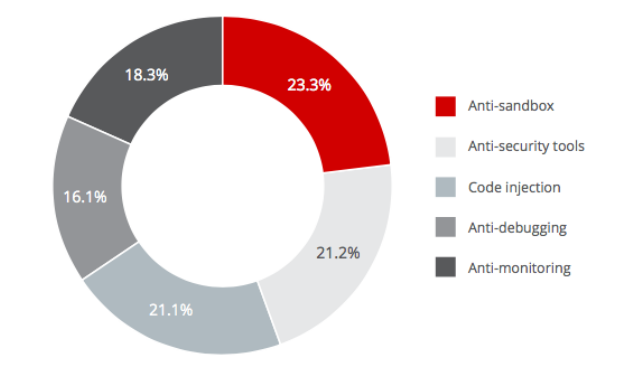
\includegraphics[width=\textwidth]{evasion_techniques_used_by_malwares_amro2018malware.png}
		\caption{Pie chart of evasion techniques \cite{amro2018malware}}
		\label{fig:pie_evasion}			
	\end{figure}
	
	
	\paragraph{} We create the below list with the help of \cite{vidas2014evading} \cite{sophos_anti_emulation} and with our own experience. We also implemented some of easier to implement tests and will talk about it in the next section. \cite{ares} implemented different evasion techniques into 22 samples and for those samples please refer to their paper.
		
	\begin{enumerate}
		\item Reading telephone number \cite{sophos_anti_emulation} \cite{vidas2014evading}
		\item Mobile country code \cite{vidas2014evading}
		\item Build.Host property \cite{sophos_anti_emulation} \cite{vidas2014evading}
		\item Build.Fingerprints property \cite{sophos_anti_emulation}\cite{vidas2014evading}
		\item Reading device IMEI number
		\item Network address e.g. 10.0.0.2/24 and routing table (netH) \cite{vidas2014evading}
		\begin{enumerate}
			\item virtual router (address space: 10.0.2/24)
			\item Emulated network (IP address: 10.0.2.15)
		\end{enumerate}
		\item Checking device uptime
		\item Checking ping example.com
		\item CPU serial number mostly in 0's \cite{vidas2014evading}
		\item CPU frequency files absent \cite{vidas2014evading}
		\item Number of sensors (SensorManager API) \cite{vidas2014evading}
		\item Bluetooth not present \cite{vidas2014evading}
		\item Battery level \cite{vidas2014evading}
		\item Checking for Manufacturer related software which comes pre-installed \cite{vidas2014evading}
		\item Checking for other usage related data e.g image, sms, calls, WLAN networks, browser history, installed applications e.g facebook etc.
		\item Checking for Google internet services \cite{vidas2014evading}
		\item Checking for marketplace application \cite{vidas2014evading}
		\item Checking for carrier added applications \cite{vidas2014evading}
		\item Delaying execution \cite{sophos_anti_emulation}
		\item Detecting lack or abundance of use input
		\item Checking if Qemu can handle interrupt while executing blocks \cite{sophos_anti_emulation}
		\item isUserMonkey(), setRunAsMonkey(false) in Android API
		\item Checking other network configurations
		\item Using native code to detect Qemu based detection in CPU implementations like some bugs
		\item CPU Performance \cite{vidas2014evading}
		\item GPU performance (Low FPS, Large variation(May not work with new emulators because of improved integration)) \cite{vidas2014evading}
		\item Input from sensors is not spread enough \cite{vidas2014evading}
		\item Camera detection \cite{vidas2014evading}
		\item Checking for Superuser.apk
		\item Checking for some specific applications with package names  \cite{vidas2014evading}
		\item Checking for apps which run only on rooted devices, e.g, busybox, executing su and id command, \cite{vidas2014evading}
		\item Checking for files e.g, /system/bin/,/system/xbin/,/sbin/. Or searching them in \$PATH (manually or by which "file")
		
		\item File permissions: Some rooting tools make certain root folders readable (e.g.,/data) or writable (e.g., /etc, /system/xbin, /system, /proc,/vendor/bin) to any process on the device. The File.canRead and File.canWrite Java APIs, or access C API can be used to check whether such condition exists.
		\item Shell Command Execution: Applications can use Runtime.exec Java API, ProcessBuilder Java class, or execve C API to execute a specific command in a separate process, and then examine the output of the shell command to detect rooting traits. Commonly employed shell commands are:
		\begin{enumerate}
			\item su: If the su binary exists, this shell command will exit without error; otherwise, an IOException will be thrown to the calling application.
			\item which su: This check involves executing the Linux ”which” command with parameter “su” and verifying if the result is 0 (indicating the su binary was found). This is essentially the same as parsing the PATH variable, but requires less work for the caller.
			\item id: This check is based on executing the command ”id”, and verifying the UID to determine if it corresponds to root (uid=0 is root)
		\end{enumerate}
	
	\item System Mounted: Normally the “/system” partition on an Android device is mounted “ro” (read only). Some rooting methods require this partition to be remounted “rw” (read-/write). There are mainly two variants of this check. The first simply runs the mount command and looks for a “rw” flag. The second attempts to create a file under “/system/” or “/data/”. If the file is successfully created, it implies the mount is “rw”.
	\item Ability to mount: This method attempts to mount the “/system” partition with the command “mount -o remount,rw /system”, and then checks if the return code was 0.
	\item Check Processes/Services/Tasks: This check consists of finding whether a specific application that requires root privileges is running on the device. The ActivityManager.getRunningAppProcesses method returns a list of currently running application processes. Similarly, getRunningServices or getRecentTasks APIs are also used by applications to retrieve a list of current running services or tasks.
	\item System properties: If the value of system property ro.secure equals “0”, the adb shell will be running as root instead of shell user. System.getProperty Java API can be used by applications to examine this property value. In addition, examining ADB source code reveals that the adbd daemon is also running as root user if both “ro.debuggable” and “service.adb.root” properties are set to ”1”.\cite{sophos_anti_emulation} \cite{vidas2014evading}
	\item hooking detection: Detecting hooks using call stack analysis \cite{lim2016android}
	\item Check debugger and installer: This one is not an anti-emulator but its purpose is also to obstruct the dynamic analysis. Like this skinner adware reported by checkpoint \cite{skinner_adware}, it uses Debug.isDebuggerConnected() and Debug.waitingForDebugger() to check if a debugger exists. More interesting, it also gets the installer using getInstallerPackageName and sees if it’s installed by Google Play (com.android.vending). So if you install the program to a device with adb, like most analysts do, the application won’t work.\cite{sophos_anti_emulation}
	
	
	\end{enumerate}
	\section{Emulator testing app}\label{sec::emulator_testor}
	After collection information about how emulator detection works, we wanted to make an app which can help us test emulators against evasion techniques so we decided to implement some of these techniques in a very simple app. Below is the list of techniques that we implemented. 
	
	\begin{itemize}
		\item read Build information
		\begin{itemize}
			\item Build.FINGERPRINT
			\item Build.HOST
			\item Build.HARDWARE
			\item Build.PRODUCT
			\item Build.MODEL
		\end{itemize}
		\item Getting stack trace to check for abnormal calls
		\item Writing to a file
		\item Getting network information
		\begin{itemize}
			\item Is wifi connected
			\item Is mobile network connected
			\item Get information related to connected network
		\end{itemize}
		\item Get Phone data
		\begin{itemize}
			\item Phone number
			\item Country
			\item getDeviceID
		\end{itemize}
		\item Checking for Root using RootBeer \cite{rootbeer}
		\item Pinging www.example.com
		\item Trying to get the IP address of the phone for all interfaces
	\end{itemize}
	\paragraph{} Our app will print the result of these tests on the screen. The screenshots of our app can be seen in figure \ref{fig:no_hooking_execute} and figure \ref{fig:hooking_execute}. Figure \ref{fig:no_hooking_execute} shows result when the method "getPhone" is not hooked. Also notice the absence of Bluetooth device, device uptime, ping result, device ID and rootbeer showing that device is rooted. In the next chapter we will explain the output of this app in more details along with introduction to another instrumentation tool called "Frida".
		\begin{figure}
			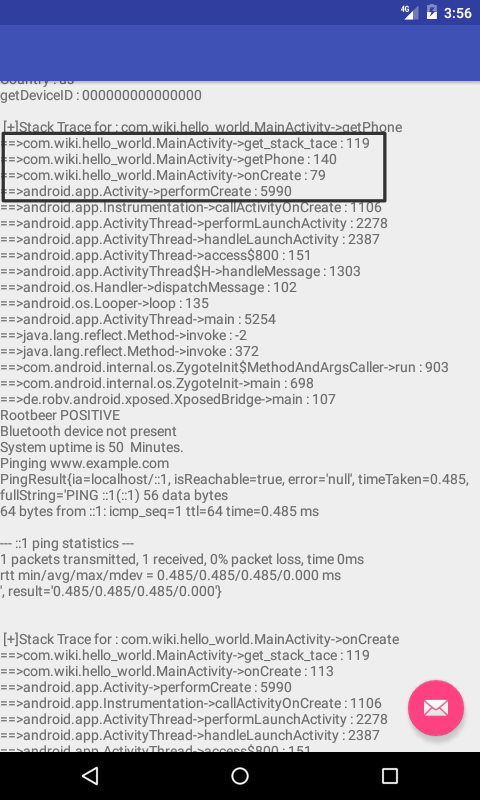
\includegraphics{hello_world_no_hooking.png}
			\caption{Executing our test app without hooking "getPhone"}
			\label{fig:no_hooking_execute}			
		\end{figure}
		
		\begin{figure}
			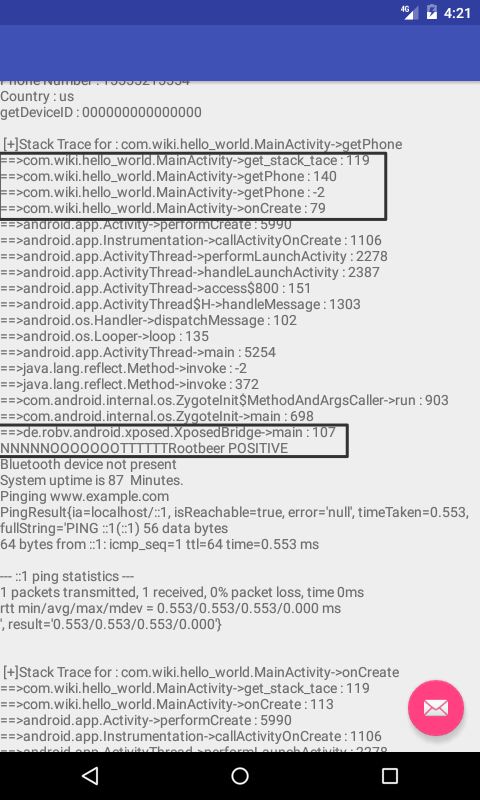
\includegraphics[width=\textwidth]{hello_word_after_hooking.png}
			\caption{Executing our test app with hooking  "getPhone"}
			\label{fig:hooking_execute}			
		\end{figure}	
	
	
	\section{Malwares that uses Anti-Emulator detection}
	\todo[inline]{Probably move to appendix}
	The purpose of this list is to help other researchers who are looking for samples that uses anit-emulation detection.
	\begin{itemize}
		\item 0ef01f50b829355b73418adcb30b20a3a1f6cb95123afce2c5469cdb25c7f7d0 Skinner
		\item 9AB5A05BC3C8F1931A3A49278E18D2116F529704 (Android/TrojanDropper.Agent.BKY) Uses delayed execution \cite{eset_multi_stage_malware}
		\item 2E47C816A517548A0FBF809324D63868708D00D0 (Android/TrojanDropper.Agent.BKY) Uses delayed execution \cite{eset_multi_stage_malware}
		\item DE64139E6E91AC0DDE755D2EF49D60251984652F (Android/TrojanDropper.Agent.BKY) Uses delayed execution \cite{eset_multi_stage_malware}
		\item 6AB844C8FD654AAEC29DAC095214F4430012EE0E (Android/TrojanDropper.Agent.BKY) Uses delayed execution \cite{eset_multi_stage_malware}
		\item C8DD6815F30367695938A7613C11E029055279A2 (Android/TrojanDropper.Agent.BKY) Uses delayed execution \cite{eset_multi_stage_malware}
		\item 47442BFDFBC0FB350B8B30271C310FE44FFB119A (Android/TrojanDropper.Agent.BKY) Uses delayed execution \cite{eset_multi_stage_malware}
		\item 604E6DCDF1FA1F7B5A85892AC3761BED81405BF6 (Android/TrojanDropper.Agent.BKY) Uses delayed execution \cite{eset_multi_stage_malware}
		\item 532079B31E3ACEF2D71C75B31D77480304B2F7B9 (Android/TrojanDropper.Agent.BKY) Uses delayed execution \cite{eset_multi_stage_malware}
	\end{itemize}
	\section{Chapter Conclusion}
	
			
\end{document}